
\chapter{LED與PD三維相對位置演算法}
\label{chp:3}

如第二章所述,LED與PD量測系統以多個LED與PD所組成,透過$P$個PD分別量測到$L$個LED的$L\times P$個量測訊號,由傳遞強度模型回推位置資訊。

本論文目標是提供一方法進行由LED與PD量測的三維定位方法,並分析調整LED與PD的擺設方法以及朗博次方對誤差的影響,進而針對不同使用情境提供最佳的系統組態。首先,會介紹LED與PD的定位系統如何運作,介紹本論文所提出的三維定位方法,在第四章介紹最佳化問題,並於第五章舉例並給出最佳系統組態。

\begin{figure}[ht]
    \centering
    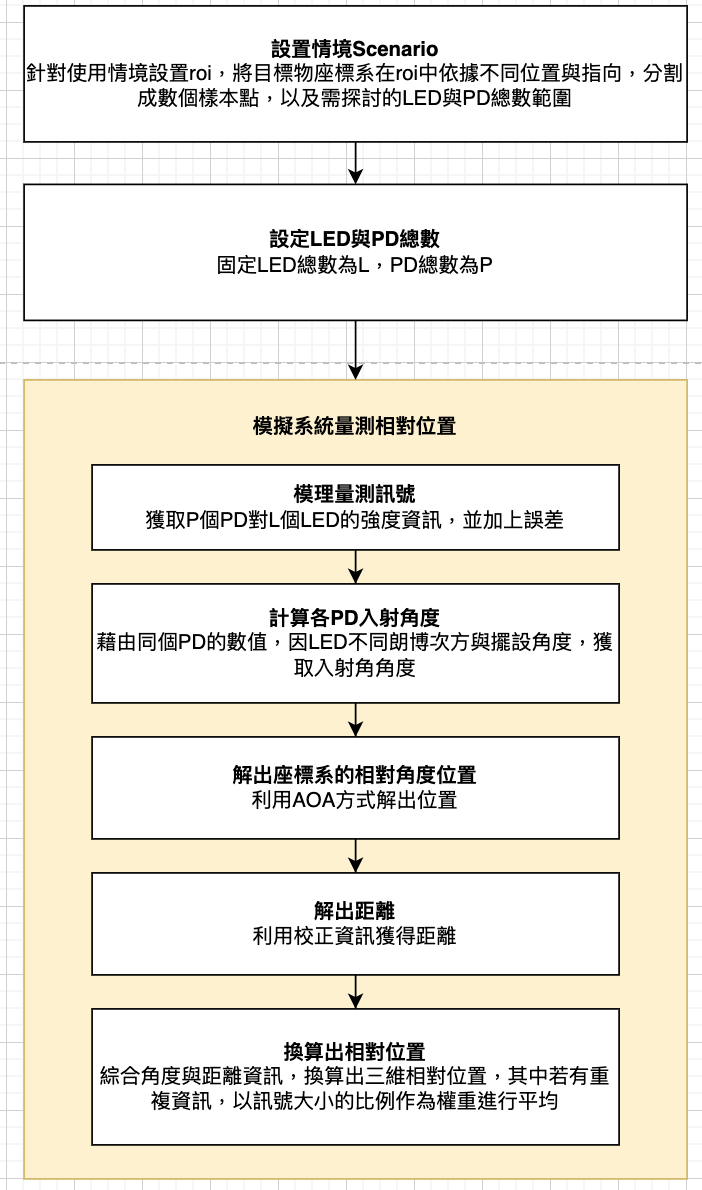
\includegraphics[width=12cm]{ch3pic/flowchart_pos.png}
    \caption{量測三維相對位置流程圖}
    \label{flow:pos}
\end{figure}



\section{系統概述}


系統組成是由多個LED與多個PD組成,PD唯一可獲得的資訊是電流大小,而PD電流大小為光強度的函數,在飽和強度以下光強度與電流成正比。多LED與多PD的互動下,每個PD都有可能收到多個LED的訊號,透過光通訊,由LED利用驅動器編碼,傳遞到PD後再進行解碼,將不同LED來源分離,得到各LED對各PD的訊號強度。


如第二章所述,PD所接收的光電流強度除了硬體參數以外,變數有三個:光於PD的入射角、光從LED的出射角、LED與PD的距離。考慮LED與PD在空間中的擺放方式,固定其中一者而另一者進行旋轉時,僅會改變出射角或是入射角,但凡兩者之間的相對位置有所改變,則同時會改變出入射角以及距離。

\begin{equation}
    \Phi_{lp}=\frac{ A_p\cos\phi_{lp}^{m_{p}} }{D^2_{lp}}\times Pt_l\frac{(M_{l}+1)}{2 \pi} \cos \theta_{lp}^{M_{l}}  \\
    =k_{lp}\frac{{\cos\theta_{lp}}^{M_{l}}{\cos\phi_{pl}}^{m_{p}}}{D_{lp}^2}\\
\end{equation}

因此,當有$L\times P$訊號強度時,每個訊號強度都是三個變數函數,為了降低方程式複雜度,最常見的方法是如上述,就是限制同一組的PD的擺設方法為僅能擺放於同個位置,這樣光強度的唯一變數僅剩下入設角度。
常見的系統設置大多是利用可見光,將定位用的LED同時當作室內光源照射,而且常見的系統是將LED與PD的中心軸限制為必須平行,例如在室內時將手機平放,內鏡頭便會垂直朝上與垂直地面朝下的LED平行。此種限制是為了更進一步的降低方程式的複雜度,使得入射角與出射角的角度相等,則可較為簡單的藉由不同的算法將定位計算出來。

然而限制兩中心軸平行的方式會極大的限制使用情境,基本上僅有在室內光源固定的狀況下較好判斷LED中心軸的方向,才能進而將接收子PD擺放至合適的接收姿態,如手機室內定位的例子,使用者移動時需全程手持手機並將其保持水平向上,大大限制了使用者的自由性。然而我們的目標情境是並沒有限制目標物的環境與相對姿態的,過去文獻的這類型演算法顯然不適用,我們需要有更加靈活不受限的演算法來解出兩者的相對定位,而本章節將提出一種符合此需求的方法。

\section{定位演算法}

本論文提出個演算法藉由多PD的訊號獲得入射角方位,再藉由多LED的訊號獲得出射角方位,綜合前兩著資訊來取得距離。

\subsection{取得入射角方位}

首先,三維定位在解析時大致分成兩種方式,一種是以卡式座標系的方式求$xyz$三者的分量,另一種常見的則是以方位(二維)與距離(一維)來解析,也可以看成是球座標系的表示方法,而接下來都會以方位與距離來解相對位置,其較直觀的將相對位置以載具的出發點分析,且一個單位的接收子或發射子剛好可以視為球座標系的中心點。

以球座標系來看,為了簡化方程式複雜度,我們同樣將所有PD擺設於同個位置,僅通過調整擺放的朝向來改變入射角度,P個PD的強度公式如下,在各PD硬體相同時,唯一的變數就是入射角度,而透過將兩兩強度相除並將已知的朗博次方的影響去除,即可獲得各PD之間的強度比值,也就是入射角的cosine比值,而在座標系中滿足入射角cosine比值的所有點皆位於同個平面上,為了方便用內積計算cosine,此段以卡式座標系表示。
而各個PD的指向可以用球座標系的天頂角與方位角$\alpha\beta$表示。

當兩PD位於原點,指向分別以$V$表示,目標物所在的方位則以小標T表示,因此可將入射角度的cosine比值寫為以下形式:

\begin{equation}
    ratio_{12}=R_{12}=\left(\frac{\Phi_{l1}}{\Phi_{l2}}\right)^{1/m_p}
    \end{equation}

式子整理過後可以看出:滿足此入射角cosine比值的目標物所在方位,為一通過原點的平面,可以透過式子描述。
\begin{equation}
    R_{12} =\frac{ \cos(\text{angle difference beween }^{P}V_1,^{P}V_L)}{\cos(\text{angle difference beween }^{P}V_2,^{P}V_L)} \\
    =\frac{^{P}V_1\cdot^{P}V_L}{^{P}V_2\cdot^{P}V_L}
\end{equation}
\begin{equation}
    ^{P}x_p(^{P}x_1-R_{12}^{P}x_2)+^{P}y_p(^{P}y_1-R_{12}^{P}y_2)+^{P}z_p(^{P}z_1-R_{12}^{P}z_2)=0
\end{equation}

$(^{P}x_1-R_{12}^{P}x_2,^{P}y_1-R_{12}^{P}y_2,^{P}z_1-R_{12}^{P}z_2)$

\subsubsection{多個平面求交軸即為解}

在上一小節中,先求三維的相對位置中的方位,透過同位置不同指向的兩PD,計算光強度的比值得到入射角的cosine比值,而滿足該比值的入射方位在座標系中維一通過原點的平面。

透過同樣方式,利用P個PD各自兩兩比較,即可得到$P-1$組通過原點的平面,求平面最簡單的方式便是利用平面法向量內積,即可獲得目標物方位。

\subsubsection{多解平均}

在一個LED對$P$個PD的系統中,將PD擺放於座標系原點而指向皆不同,去除掉可視範圍外的PD,共有$P_u$(代表usable)個強度訊號,取一強度訊號作為參考強度,將其他$P_u-1$個強度訊號與參考強度相除並去除朗博次方的影響,即可獲得$P_u-1$個目標方位可能存在的平面。將$P_u-1$個平面中的其中一個平面同樣當作參照,即可將另外的$P_u-2$與其進行外積得到$P_u-2$個解,則最少需要有三個有訊號的PD才能得到解。

\begin{equation}
    ^{PL}\hat{\boldsymbol{T}} = 
    \sum_{i=1}^{P_u-2} (\vec{n_{r}}\times\vec{n_{i}})
\end{equation}

\begin{figure}[ht]
    \centering
    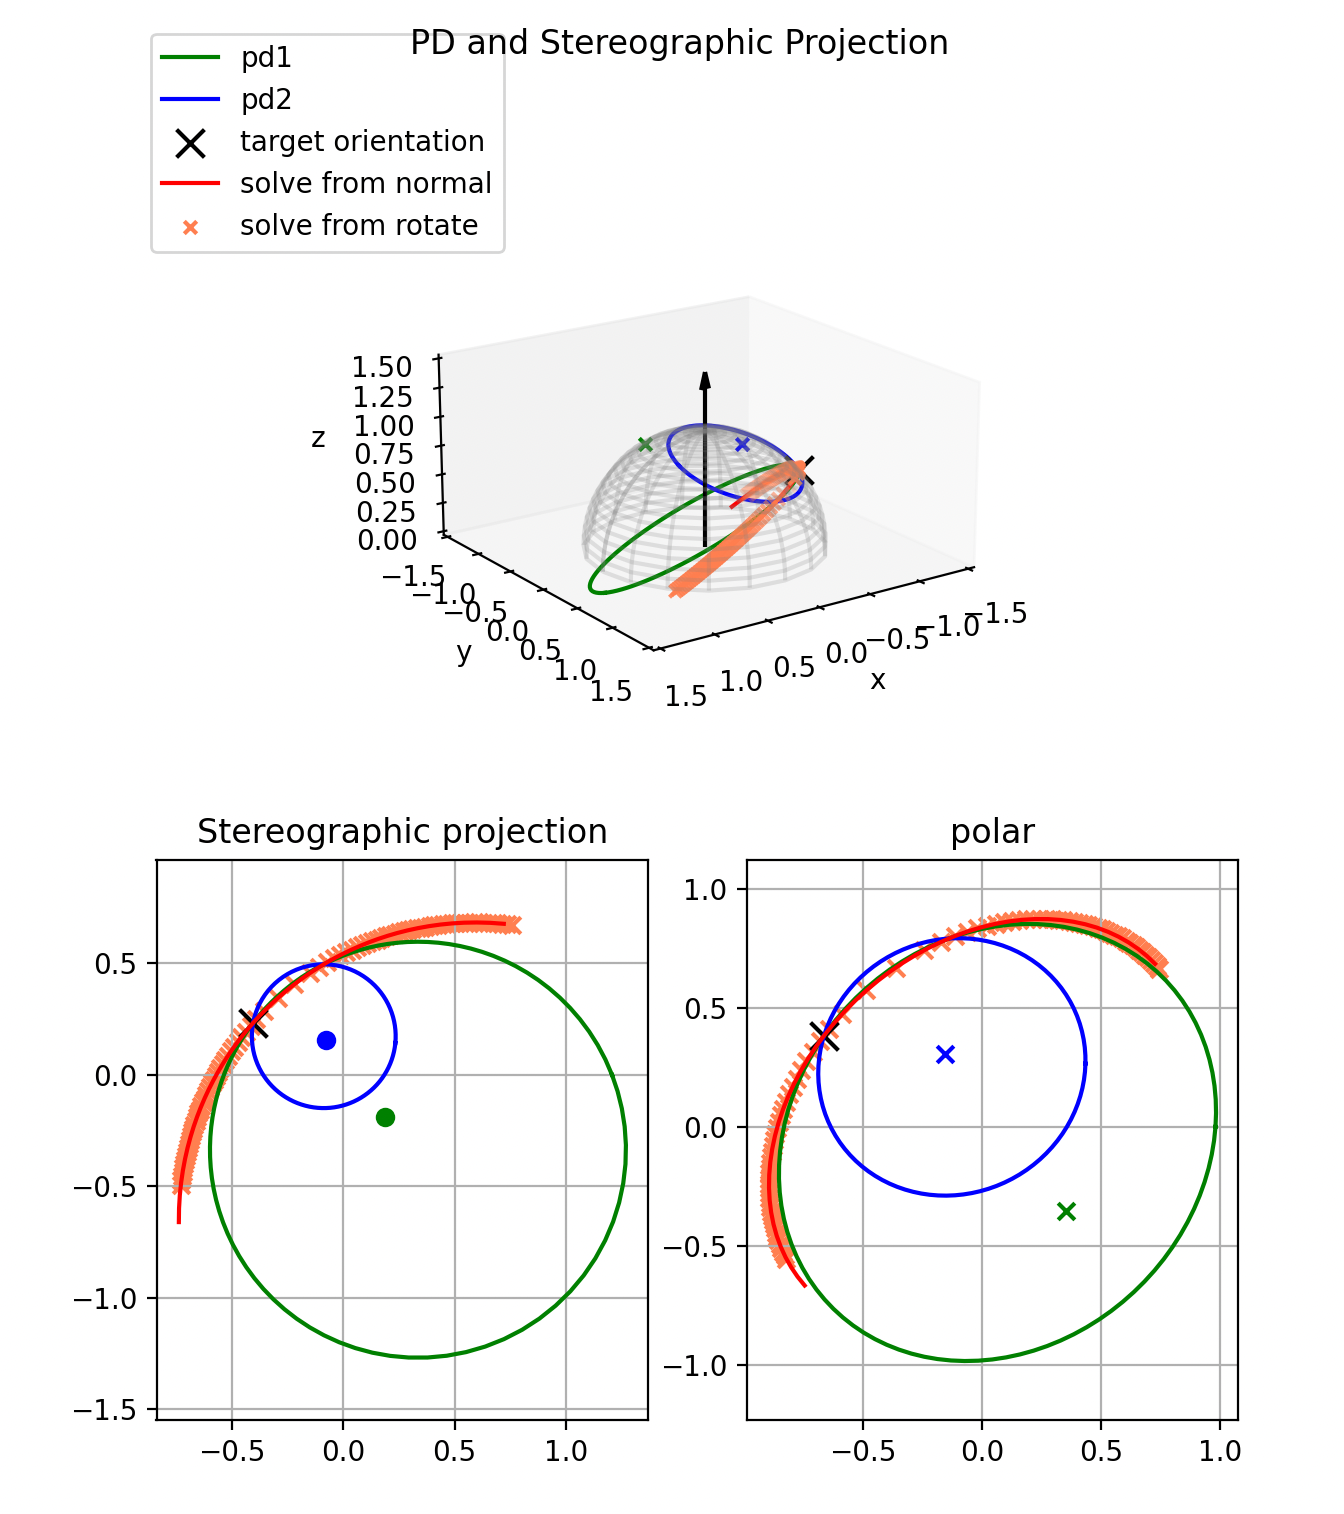
\includegraphics[width=12cm]{ch3pic/solve_targetori.png}
    \caption{演算法結果}
    \label{solve_ori}
\end{figure}


\subsection{取得距離}

藉由單個LED與三個以上接收到訊號的PD,即可獲得入射角方位(二維)的資訊,欲獲得距離之前,則需將LED出射角資訊獲得。而LED出射角資訊可以利用與PD入射角資訊相同的方式取得,只是改成多個LED對單個PD的訊號量測,藉由比較同個PD所收到不同LED的訊號比值獲得。


求出入射角與出射角方位之後即可從光傳遞模型推算出距離。

\section{誤差分析}
